\documentclass[10pt]{article}

%==============================
% Document Metadata
%============================== 
\usepackage[pdftex,
    pdfauthor={Rukmal Weerawarana},
    pdftitle={Homework 1 Solutions - FE 621},
    pdfsubject={FE 621 - Computational Methods in Finance}
]{hyperref}


%==============================
% Package Imports
%==============================    
\usepackage[ruled]{algorithm2e}
\usepackage[authordate, maxcitenames=1]{biblatex-chicago}
\usepackage{amsmath} % math environment stuff
\usepackage{amssymb} % additional math symbols
\usepackage[toc, page]{appendix} % Appendix referencing
\usepackage{comment} % enables the use of multi-line comments (\ifx \fi) 
\usepackage{csvsimple} % CSV to Table
\usepackage{fancyhdr} % Header
\usepackage{fancyvrb}
\usepackage{float}
\usepackage[headings]{fullpage}
\usepackage{graphicx}
\usepackage{listings} % code embedding
\usepackage{pmboxdraw}
\usepackage[dvipsnames]{xcolor} % colors for code


%==============================
% Configuration
%==============================

% Figure outline configuration
\floatstyle{boxed}
\restylefloat{figure}

% Bibliography configuration

\addbibresource{../bibliography.bib}

% Remapping bibliography underscores (_) and tildes (~) because Mendeley has weird exporting
% Solution from: https://tex.stackexchange.com/questions/309980/parsing-underscores-in-urls-from-mendeley

\DeclareSourcemap{ % Used when .bib/Bibliography is compiled, not when document is
    \maps{
        \map{ % Replaces '{\_}', '{_}' or '\_' with just '_'
            \step[fieldsource=url,
                  match=\regexp{\{\\\_\}|\{\_\}|\\\_},
                  replace=\regexp{\_}]
        }
        \map{ % Replaces '{'$\sim$'}', '$\sim$' or '{~}' with just '~'
            \step[fieldsource=url,
                  match=\regexp{\{\$\\sim\$\}|\{\~\}|\$\\sim\$},
                  replace=\regexp{\~}]
        }
    }
}

% Code display configuration

\newcommand*\lstinputpath[1]{\lstset{inputpath=#1}} % Setting path
\lstset{
	language=Python,
	basicstyle=\footnotesize\ttfamily,
	commentstyle=\ttfamily\color{purple!40!black},
	identifierstyle=\color{blue},
	keywordstyle=\color{ForestGreen},
	numbers=left,
	numberstyle=\ttfamily\color{gray}\footnotesize,
	stepnumber=1,
	numbersep=5pt,
	backgroundcolor=\color{white},
	showspaces=false,
	showstringspaces=false,
	showtabs=false,
	frame=single,
	tabsize=2,
	captionpos=b,
	breaklines=true,
	breakatwhitespace=false,
	title=\lstname
}
\lstset{
	language=R,
	basicstyle=\footnotesize\ttfamily,
	commentstyle=\ttfamily\color{purple!40!black},
	identifierstyle=\color{blue},
	keywordstyle=\color{ForestGreen},
	numbers=left,
	numberstyle=\ttfamily\color{gray}\footnotesize,
	stepnumber=1,
	numbersep=5pt,
	backgroundcolor=\color{white},
	showspaces=false,
	showstringspaces=false,
	showtabs=false,
	frame=single,
	tabsize=2,
	captionpos=b,
	breaklines=true,
	breakatwhitespace=false,
	title=\lstname
}

% Header and Footer configuration

\pagestyle{fancy} % set page style
\fancyhead{} % override header
\fancyfoot{} % override footer
\renewcommand{\headrulewidth}{.4pt} % set header rule width 
\renewcommand{\footrulewidth}{.4pt} % set footer rule width 
\lhead{Homework Assignment 1} % set left header
\rhead{Rukmal Weerawarana} % set right header
\lfoot{\textit{FE 621}: Computational Methods in Finance} % set left footer
\rfoot{Page \thepage} % set right footer


%==============================
% Document Content
%==============================

\begin{document}

\thispagestyle{plain}

%==============================
% Document Title
%==============================

\noindent
\large\textbf{Homework Assignment 1} \hfill \textbf{Rukmal Weerawarana} \\
\normalsize \textit{FE 621}: Computational Methods in Finance \hfill \textit{rweerawa@stevens.edu} $\mid$ 104-307-27 \\
\textit{Instructor}: Ionut Florescu \hfill Department of Financial Engineering \\
2/20/2019 \hfill Stevens Institute of Technology

\noindent\rule{\linewidth}{.1em}


%==============================
% Overview
%==============================

\section*{Overview}

In this Homework Assignment, we explore various numerical optimization methods through the lens of the Black-Scholes-Merton Option pricing model (\cite{Shreve2004}). Using this, we calculate explore the implied volatility of options for various assets traded on the market. Furthermore, we also explore numeric methods of differential calculation to compute the Greeks of these candidate options. Finally, we explore numeric integration and the behavior of various quadrature methods.

Unless otherwise stated, the following shorthand notation is used to distinguish between dates:

\begin{itemize}
    \item \textbf{DATA1} - Wednesday, February 6 2019 (\textit{2/6/19})
    \item \textbf{DATA2} - Thursday, February 7 2019 (\textit{2/7/19})
\end{itemize}

The content of this Homework Assignment is divided into three sections; the first discusses data gathering, formatting, and a discussion of the assets being examined. The second contains data analysis, and an exploration of implied volatility through the Black-Scholes-Merton pricing framework and related computations. Finally, the third section discusses numerical integration and the convergence of various quadrature rules.

\begin{center}
    \textit{See Appendix \ref{appendix:source} for specific question implementations, and (\cite{Weerawarana2019}) for full source code of the {\normalfont fe621} Python package.}
\end{center}


%==============================
% Section 1
%==============================

\newpage

\section{Data Overview}

    \subsection{Asset Descriptions}

        \subsubsection{\textit{SPY} - SPDR S\&P 500 ETF (\cite{StateStreetGlobalAdvisors2019})}

        The S\&P 500 (i.e. \textit{Standard \& Poor's 500}) is a stock market index tracking the 500 largest companies on the American Stock Exchange by Market Capitalization. In this case, the market capitalization is defined as the number of outstanding shares, multiplied by the current share price. A stock market index is designed to be a metric that can be used by market observers as a benchmark to gauge the relative health of the stock market, by analyzing the aggregate performance of its largest components.
            
        However, this index is not the same as the \textit{SPY} ETF. An ETF (\textit{Exchange Traded Fund}) is a basket of stocks that is designed to track a specific index or benchmark. That is, it provides investors with exposure to a index or benchmark, without having to own all of the underlying assets that constitute a composite ETF. In addition to higher liquidity, this type of investment also provides lower transaction costs and required minimum investment to gain exposure to a given index or benchmark. It is traded on an exchange, akin to a typical traded asset.

        \subsubsection{\textit{VIX} - CBOE Volatility Index (\cite{CBOEChicagoBoardOptionsExchange2019})}

        The CBOE (\textit{Chicago Board Options Exchange}) volatility index, \textit{VIX} is an exchange traded product (\textit{ETP}) designed to give investors exposure to the market's expectation of 30-day volatility. It is priced using a large set of implied volatility of put and call options on the S\&P 500 index to gauge investor sentiment. Typically, the price of the VIX has an inverse relationship to the price of the S\&P 500 index. Similar to an ETF, an ETP is also traded on an exchange as a typical traded asset.


    \subsection{Data Gathering}

    For the assignment, we downloaded monthly options on \textit{Amazon Inc.} (ticker: AMZN) and \textit{S\&P 500 ETF} (ticker: SPY) at various strike prices for the following dates:
    
    \begin{itemize}
        \item \textit{02/15/19} - Friday, February 15 2019;
        \item \textit{03/15/19} - Friday, March 15 2019;
        \item \textit{04/18/19} - Thursday, April 18 2019.
    \end{itemize}

    A wide variety of option strike prices were considered, with the following ranges:
    
    \begin{itemize}
        \item \textit{AMZN} - \$1555 to \$1725 in increments of \$5 (35 strike prices);
        \item \textit{SPY} - \$256 to \$284 in increments of \$1 (29 strike prices).
    \end{itemize}

    Intra-day minute closing price data was gathered for both put and call options with expiration dates and strike prices detailed above. This intra-day data was gathered for the trading day \textit{2/6/19} (February 6 2019; \textbf{DATA1}). Additionally, intra-day minute closing price data was also downloaded for each of the underlying assets. This data was downloaded for both \textit{2/6/19} (February 6 2019; \textbf{DATA1}), and \textit{2/7/19} (February 7 2019; \textbf{DATA2}).

    This data detailed above was gathered utilizing \textit{Rblpapi} (\cite{Armstrong2018}), which provides an R interface to data on the Bloomberg Terminal (\cite{BloombergL.P.2019}). The data download was automated, and corresponding intra-day prices for each of the options were output to individual files. The source code for this implementation is available in Appendix \ref{appendix:source:q1:bloomberg}.

    Furthermore, as a proxy for the \textit{risk-free rate}, we chose to utilize the effective Federal Funds Rate (FFR). This is the interest rate at which depository institutions in the United States lend reserve balances to other depository institutions overnight. This data was gathered for both dates, and correspond to \textbf{DATA1} and \textbf{DATA2}. The effective FFR is published daily by the US Federal Reserve Board of Governors, and are expressed as yields per annum (\cite{BoardofGovernorsoftheFederalReserveSystem2019}).

        \subsubsection{Data Cleaning}

            For easier programmatic access, the data was placed in a hierarchical structure, corresponding to the \textbf{DATA1}, \textbf{DATA2} data division. Each of the option and asset prices for the corresponding days were placed in the requisite sub-folders. This directory structure is reproduced below.

            \VerbatimInput{bin/data_tree.txt}

            Option price filenames were changed to OOC format option names, discussed further below. This was done utilizing a cleaning script, written in Python. This script employs utility functions from the \textit{fe621} Python package (\cite{Weerawarana2019}). The cleaning script is reproduced in Appendix \ref{appendix:source:q1:clean}.
    
        \subsection{Option Naming Convention}

        A modern convention for naming option contracts was proposed by the Options Clearing Commission (OCC) in 2008 (\cite{OptionsSymbologyInitiative2008}), and adopted in 2010. The OCC is an organization that acts as both the issuer and guarantor for option and future contracts. The OCC is governed by the Securities and Exchange Commission (SEC) and the Commodities Futures Trading Commission (CFTC). The current convention for option naming is best explained by example.
        
        Consider the option code, \textit{AMZN190215C01960000}. This corresponds to a \textbf{Call Option} on \textbf{Amazon Inc. (AMZN)}, with a strike price of \textbf{\$1960.00} and an expiration date of \textbf{2/15/19} (February 15 2019).
        
        The methodology of this nomenclature is explained in detail below:
    
        \begin{center}
            \textbf{\textcolor{red}{AMZN}\textcolor{MidnightBlue}{19}\textcolor{Bittersweet}{02}\textcolor{YellowOrange}{15}\textcolor{RoyalPurple}{C}\textcolor{ForestGreen}{01960}\textcolor{violet}{000}}
        \end{center}
    
        \begin{itemize}
            \item \textbf{\textcolor{red}{AMZN}} - Ticker of the company (arbitrary length; always first sequence of characters)
            \item \textbf{\textcolor{MidnightBlue}{19}} - Expiration year of the contract (shortened to two digits, i.e. 2019 $\rightarrow$ 19)
            \item \textbf{\textcolor{Bittersweet}{02}} - Expiration month of the contract
            \item \textbf{\textcolor{YellowOrange}{15}} - Expiration day of the contract
            \item \textbf{\textcolor{RoyalPurple}{C}} - Type of option (\textit{C} for call, \textit{P} for put)
            \item \textbf{\textcolor{ForestGreen}{01960}} - Dollar component of strike price (in \$; always 5 digits)
            \item \textbf{\textcolor{violet}{000}} - ${\frac{1}{1000}}^\text{th}$ Dollar component of strike price (in $\frac{1}{1000}$\$; always 3 digits)
        \end{itemize}
    
        Similarly, the following option code corresponds to a \textbf{Put Option} on \textbf{SPDR S\&P 500 ETF (SPY)}, with a strike price of \textbf{\$287.50} and an expiration date of \textbf{3/15/19} (March 15 2019):
    
        \begin{center}
            \textbf{\textcolor{red}{SPY}\textcolor{MidnightBlue}{19}\textcolor{Bittersweet}{03}\textcolor{YellowOrange}{15}\textcolor{RoyalPurple}{P}\textcolor{ForestGreen}{00287}\textcolor{violet}{500}}
        \end{center}
    
        Finally, the following option code corresponds to a \textbf{Call Option} on \textbf{CBOE Volatility Index (VIX)}, with a strike price of \textbf{\$16.35} and an expiration date of \textbf{4/18/19} (February 18 2019):
    
        \begin{center}
            \textbf{\textcolor{red}{VIX}\textcolor{MidnightBlue}{19}\textcolor{Bittersweet}{04}\textcolor{YellowOrange}{18}\textcolor{RoyalPurple}{C}\textcolor{ForestGreen}{00016}\textcolor{violet}{350}}
        \end{center}


%==============================
% Section 2
%==============================

\newpage

\lstinputpath{..}

\section{Data Analysis}

    \begin{center}
        \textit{Note: All Python scripts reproduced in this section are extracted from the {\normalfont fe621 (\cite{Weerawarana2019}}) package created for this class.}
    \end{center}

    \subsection{Black-Scholes Model Formulas}

    With the probabilities $d_1$ and $d_2$ defined as:
    \begin{gather*}
        d_1 = \frac{\log \left( \frac{S_t}{K} \right) + \left( r + \frac{\sigma^2}{2} \right) (T-t)}{\sigma \sqrt{T-t}} \\
        d_2 = d_1 - \sigma \sqrt{T-t} \\
        \Phi(x) = \int_{-\infty}^{x} \phi(z) dz = \int_{-\infty}^{x} \frac{1}{\sqrt{2\pi}} e^{\frac{-z^2}{2}} dz
    \end{gather*}

    \lstinputlisting{fe621/black_scholes/util.py}

    \begin{center}
        \textbf{\textit{Note:} The following assumes the dividend rate, $q = 0$.}
    \end{center}

        \subsubsection{Put Option}

        The Black-Scholes Option price for a European Put ($P(S_t)$) option is defined as:
        \begin{gather*}
            P(S_t) = K e^{-r(T-t)} \Phi(-d_2) - S_t \Phi(-d_1)
        \end{gather*}

        \lstinputlisting{fe621/black_scholes/put.py}


        \subsubsection{Call Option}

        The Black-Scholes Option price for a European Call ($C(S_t)$) option is defined as:
        \begin{gather*}
            C(S_t) = S_t \Phi(d_1) - K e^{-r(T-t)} \Phi(d_2) \\
        \end{gather*}

        \lstinputlisting{fe621/black_scholes/call.py}


        \subsubsection{Put-Call Parity}

        The relationship between the price of a Call and Put option is governed by Put-Call parity:
        \begin{gather*}
            P(S_t) = C(S_t) - S_t + K e^{-r(T-t)}
        \end{gather*}
    
        \lstinputlisting{fe621/black_scholes/parity.py}


        \subsubsection{The Greeks}

        The Greeks are the quantities representing the sensitivity of the price of a derivative with respect to changes in the underlying parameters. The following formulas are implemented to calculate each of the Greeks using the Black-Scholes option pricing formula. These formulas are derived in full in \cite{Stefanica2011} and \cite{Weerawarana2016}.

        \begin{center}
            \textbf{\textit{Note:} The following assumes the dividend rate, $q = 0$.}
        \end{center}
    
        \textbf{Delta}
    
        The Delta ($\Delta$) of an option is the first derivative of an option with respect to the price of the underlying asset at time $t$, $S_t$.
    
        \begin{gather*}
            \Delta(C) = \frac{\partial C(S_t)}{\partial S_t} = \Phi(d_1)
        \end{gather*}
    
        \textbf{Gamma}
    
        The Gamma ($\Gamma$) of an option is the second derivative of an option with respect to the price of the underlying asset at time $t$, $S_t$.
    
        \begin{gather*}
            \Gamma(C) = \frac{\partial^2 C(S_t)}{\partial S_t^2} = \frac{\phi(d_1)}{S_t \sigma \sqrt{T-t}}
        \end{gather*}
    
        \textbf{Vega}
    
        The Vega ($\nu$) of an option is the first derivative of an option with respect to the volatility of the underlying asset at time $t$, $\sigma$.
        
        \begin{gather*}
            \nu(C) = \nu(P) = \frac{\partial C(S_t)}{\partial \sigma} = S_t \sqrt{T-t} \, \phi(d_1)
        \end{gather*}
        
        \lstinputlisting{fe621/black_scholes/greeks.py}

    \newpage
    \subsection{Numeric Optimization}

        \subsubsection{Bisection Method}

        \begin{algorithm}[t]
            \SetAlgoNoLine
            \KwIn{Input function, $f$ to be optimized; must have sign change. Search space start and stop points, $a$ and $b$. Tolerance level, $\epsilon$.}
            \KwOut{Point $x_0$ in the interval $[a, b]$ where $f(x_0) = 0$.}
            Let midpont = $m$\;
            \Repeat{$(b - a) < \epsilon$}{
                $m = \frac{a + b}{2}$\;
                \If{$f(a) \times f(mid) < 0$}{$b=m$}
                \If{$f(b) \times f(mid) < 0$}{$a=m$}
            }
            $x_0 = \frac{a + b}{2}$\;
            \caption{Bisection Algorithm}
            \label{alg:bisection}
        \end{algorithm}

        In this section, we implement the Bisection method to compute the implied volatility, using the market price of the underlying asset and the option contract.

        The bisection algorithm is outlined in Algorithm \ref{alg:bisection}. The algorithm is implemented recursively.

        \lstinputlisting{fe621/optimization/bisection.py}


    \subsection{Implied Volatility}

    In this section, we utilize the functions and data described above to calculate the average implied volatility of each of the option chains. This was done for the entire dataset using the Bisection Method, but convergence times using the Newton Method were also explored.

    \subsection{Volatility Plots}
        \subsubsection{Volatility Smile}
        
        \begin{figure}
            \begin{tabular}{cc}
                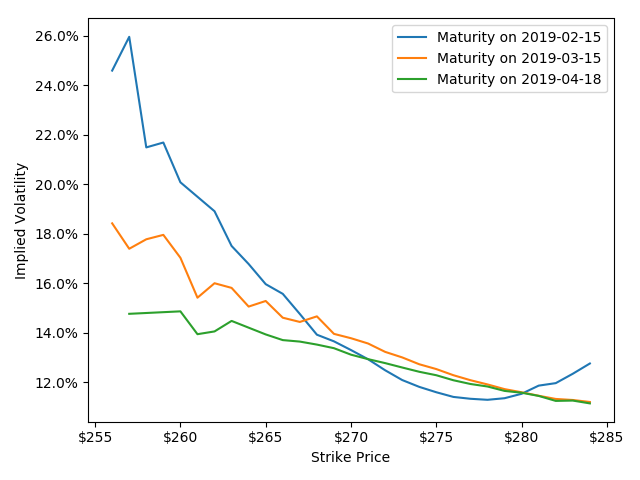
\includegraphics[width=.475\textwidth]{bin/vol_smile/SPY_Call_2DVolSmile.png} &
                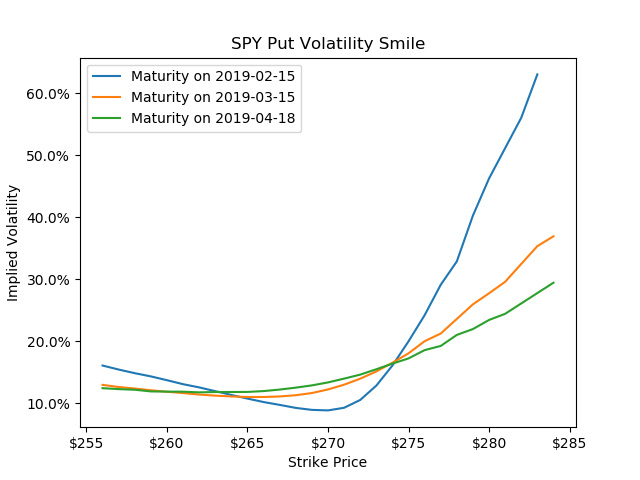
\includegraphics[width=.475\textwidth]{bin/vol_smile/SPY_Put_2DVolSmile.png} \\
                (a) SPY Call Option Volatility Smile &
                (b) SPY Put Option Volatility Smile \\
                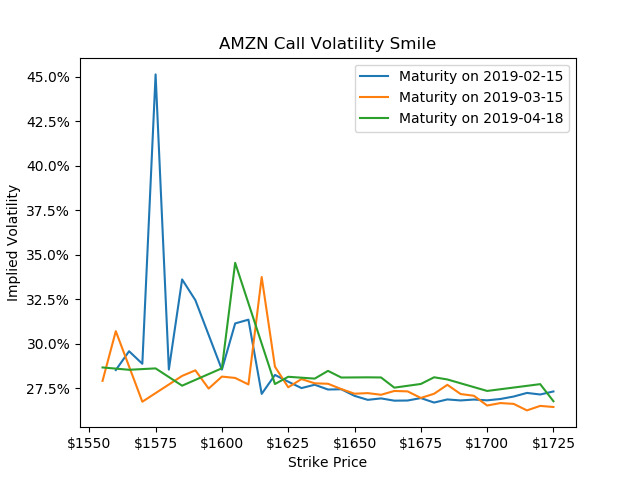
\includegraphics[width=.475\textwidth]{bin/vol_smile/AMZN_Call_2DVolSmile.png} &
                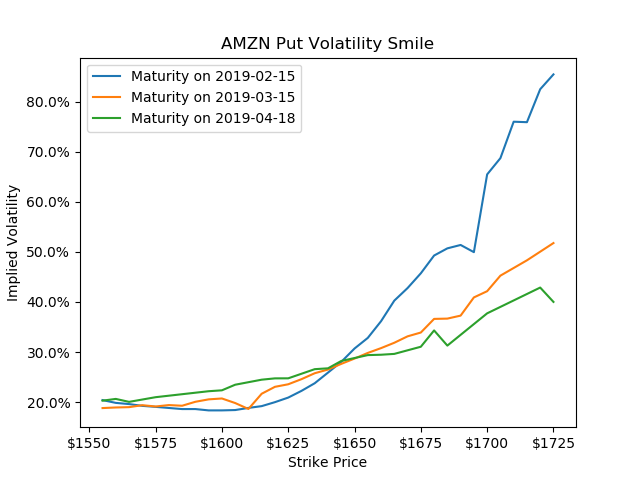
\includegraphics[width=.475\textwidth]{bin/vol_smile/AMZN_Put_2DVolSmile.png} \\
                (c) AMZN Call Option Volatility Smile &
                (d) AMZN Put Option Volatility Smile
            \end{tabular}
        \end{figure}

        \subsubsection{Volatility Surface}

        \begin{figure}
            \begin{tabular}{cc}
                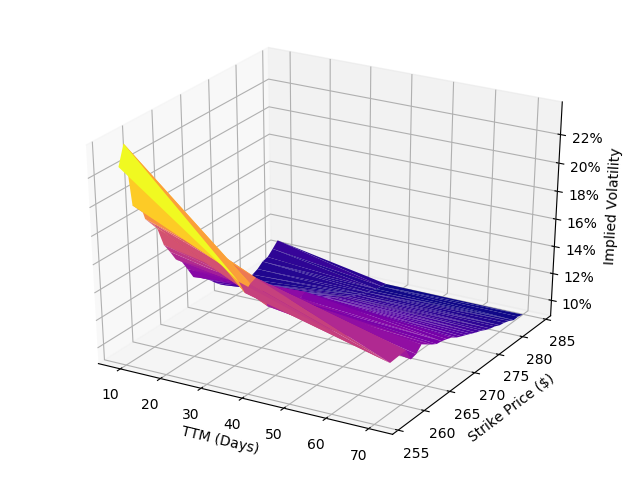
\includegraphics[width=.475\textwidth]{bin/vol_surface/SPY_Call_3DVolSurface.png} &
                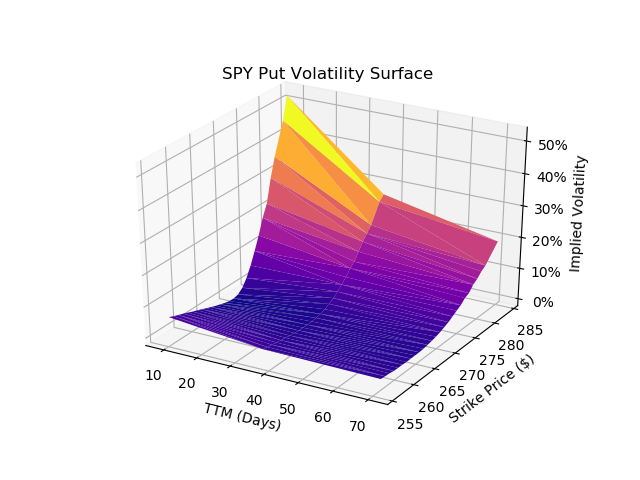
\includegraphics[width=.475\textwidth]{bin/vol_surface/SPY_Put_3DVolSurface.png} \\
                (a) SPY Call Option Volatility Surface &
                (b) SPY Put Option Volatility Surface \\
                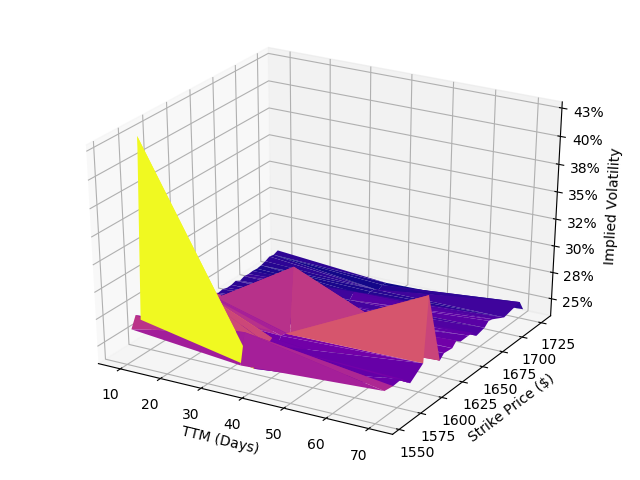
\includegraphics[width=.475\textwidth]{bin/vol_surface/AMZN_Call_3DVolSurface.png} &
                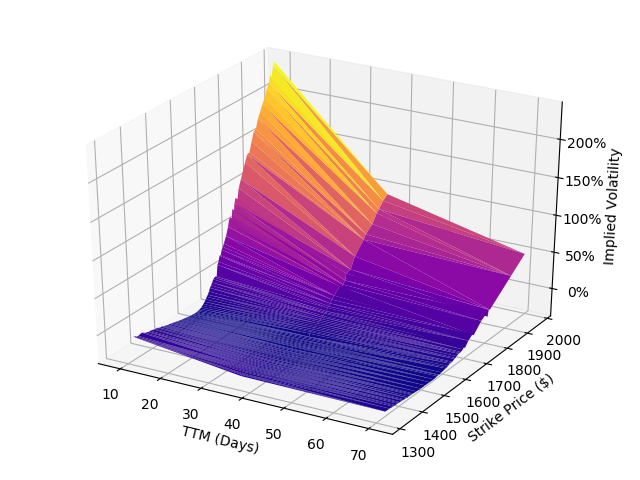
\includegraphics[width=.475\textwidth]{bin/vol_surface/AMZN_Put_3DVolSurface.png} \\
                (c) AMZN Call Option Volatility Surface &
                (d) AMZN Put Option Volatility Surface
            \end{tabular}
        \end{figure}

%==============================
% References
%==============================

\newpage

\printbibliography


%==============================
% Appendix
%==============================

\newpage

\appendix

% Resetting input path
\lstinputpath{}

\section{Appendix} \label{appendix:source}

    \subsection{Question 1 Implementation}

        \subsubsection{Bloomberg Data Download} \label{appendix:source:q1:bloomberg}

            \lstinputlisting{question_solutions/question_1.R}
        
        \subsubsection{Data Cleaning} \label{appendix:source:q1:clean}
        
            \lstinputlisting{data_cleaning.py}
    
%==============================
% Document End
%==============================

\end{document}
